\textbf{COLUNI 2023 -- Questão 38}\par\medskip Analise os documentos I, II e III.

\noindent
\begin{minipage}[t]{0.48\linewidth}
\begin{center}\textbf{Documento I}\\
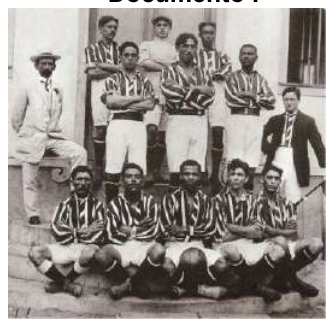
\includegraphics[width=0.75\linewidth]{static/simulados/coluni/figuras/2023/questao-38/figura-1.png}\end{center}
“No início do século XX, poucos times de futebol brasileiros aceitavam a participação de jogadores negros. O Ponte Preta, do estado de São Paulo, e o Bangu, do Rio de Janeiro, foram os primeiros times com jogadores negros. Na foto, o time do Bangu em 1911”.

CHIBA, Charles Hokiti Fukushigue, MINORELLI, Caroline Torres. \textbf{Convergências}: história, 9º ano. São Paulo: Edições SM, 2016. p. 40.
\end{minipage}\hfill
\begin{minipage}[t]{0.48\linewidth}
\begin{center}\textbf{Documento II}\\
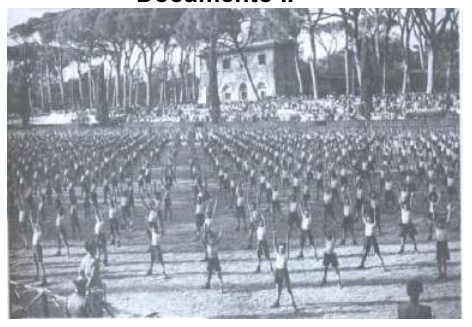
\includegraphics[width=0.95\linewidth]{static/simulados/coluni/figuras/2023/questao-38/figura-2.png}\end{center}
“Meninos da juventude fascista exercitando-se, em foto de 1936”.

Boulos Junior, Alfredo. \textbf{História}: Sociedade e Cidadania. São Paulo: FTD, 2009. p. 97.
\end{minipage}

\begin{center}\textbf{Documento III}\end{center}
\noindent
\begin{minipage}[t]{0.32\linewidth}
\begin{center}

\includegraphics[width=0.70\linewidth]{static/simulados/coluni/figuras/2023/questao-38/figura-3.png}\\
\textit{“Escudo do Palestra Italia utilizado entre 1915 e 1942.”}
\end{center}
\end{minipage}\hfill
\begin{minipage}[t]{0.64\linewidth}
“O Palestra Italia, clube de futebol de São Paulo, foi fundado em 26 de agosto de 1914 por imigrantes italianos. Com a entrada do Brasil na Segunda Guerra [...] o clube foi obrigado a mudar seu nome, passando a se chamar Palestra de São Paulo. [...] Em 20 de setembro de 1942, adotou o nome Sociedade Esportiva Palmeiras, que se mantém até hoje”.
\end{minipage}

\begin{center}BRAICK, Patrícia Ramos. \textbf{Estudar história}. Das origens do homem à era digital. São Paulo: Moderna, 2015, p. 117.\end{center}

Com base nos documentos I, II e III e nos conhecimentos históricos, é INCORRETO afirmar:
\begin{enumerate}
\item A mudança do nome do Clube Palestra Italia para Palestra de São Paulo pode ser explicada pelas
       pressões políticas e pelas contradições sociais geradas com a entrada do Brasil na Segunda Guerra
       Mundial, se posicionando ao lado dos países Aliados.
\item O futebol brasileiro, embora tenha sido utilizado como propaganda política do governo Médici, em função
       da vitória da seleção brasileira na Copa do Mundo de 1970, não sofre mais interferências de campanhas
       sociais ou de movimentos políticos.
\item O fato de os primeiros times de futebol formados no Brasil não terem tido jogadores negros evidencia o
       racismo estrutural da sociedade brasileira, que ainda é observado nos estádios esportivos brasileiros na
       contemporaneidade.
\item As festas esportivas e as demonstrações de atletismo foram utilizadas por diferentes regimes autoritários
       para criar uma imagem de sociedade alegre, harmoniosa e feliz, visando ocultar práticas repressivas e
       manter o controle social.
\end{enumerate}
